\section{Strings}

\subsection{Substrings}

\par A função substr de string retorna uma substring interna da string inicial, os parâmetros são:
\begin{itemize}
    \item Posição inicial
    \item Tamanho da substring
\end{itemize}
\par Ex: substring que remove o último char da string str.
\begin{verbatim}
    str.substr(0, str.length()-1);
\end{verbatim}

\subsection{char to int}
\begin{verbatim}
    int x = s[i] - '0';
\end{verbatim}

\subsection{int to char}
\par Para converter um int x em um char, fazemos:
\begin{verbatim}
    char c = '0' + x;
\end{verbatim}

\subsection{int to string}
\begin{verbatim}
    string str = to_string(x);
\end{verbatim}

\subsubsection{int128 to string}
Em casos muito específicos em que é necessário um inteiro de 128 bits, cout não aceita esse inteiro, para isso o convertemos em string.
\begin{verbatim}
    string to_string128(__int128_t t){
        string ans;
        while (t > 0){
            ans += ('0'+t%10);
            t /= 10;
        }
        reverse(ans.begin(), ans.end());
        return ans;
    }
\end{verbatim}


\subsection{string to int}
\begin{verbatim}
    int n = stoi(s);
\end{verbatim}


\subsection{Leitura}
Para se fazer a leitura de uma palavra, pode-se utilizar cin$>>$str. No entanto, 
esse comando não permite a leitura de uma frase, que deve ser feita utilizando 
o comando abaixo
\begin{verbatim}
    getline(cin, s).
\end{verbatim}
Além disso, sempre um cin for utilizado antes do getline, deve-se utilizando o comando
a seguir para "limpar" a entrada
\begin{verbatim}
    cin.ignore()
\end{verbatim}
Desta forma, para uma leitura no estilo t / t frases temos:
\begin{verbatim}
    int t; cin>>t; cin.ignore()
    while (t-->0){
        string str;
        getline(cin, str);
    }
\end{verbatim}
Ademais, para fazer o uso de strings com acento deve-se utilizar os comandos
\begin{verbatim}
    setlocale(LC_ALL, "pt_BR.UTF-8"); wcin; wcout; e wstring;
\end{verbatim}
Não sendo possível utilizar esses comandos separadamente ou com os comandos
básicos do template para C++.

Além disso, também há o comando stringstream, esse que por sua vez tem o objetivo de
receber uma string na construtora e acessar ela palavra/número por palavra/número.
\begin{verbatim}
    string str; getline(cin, str);
    stringstream leitura(str);
    int num;
    while(leitura >> num){nome_vector.push_back(num);}
    //Código que separa todos os números de uma string em um vector.
\end{verbatim}

\subsection{Find}
Dada uma string S e uma substring k, para descobrirmos o índice de início de k em S, 
utilizamos o seguinte comando,
\begin{verbatim}
    int pos = s.find(k);
    if (pos == npos){Não é substring}
\end{verbatim}

\subsection{KMP - String Matching}
Algoritmo Knutt-Morris-Pratt para string matching, procurar uma string \lstinline{pat} dentro
de uma string \lstinline{txt}. Complexidade: $\mathcal{O}(n+m)$


\begin{verbatim}
    
vi lps, matches;

void preKMP(string pat){
    int m = pat.length();
    lps = vi(m);
    int i = 1, len = 0;
    while(i < m){
        if (pat[i] == pat[len])
            lps[i++] = ++len;
        else if (len != 0)
            len = lps[len-1];
        else
            lps[i++] = 0;
    }
}

void KMP(string pat, string txt){
    int n, m, i = 0, j = 0;
    n = txt.length();
    m = pat.length();
    preKMP(pat);
    
    while(i < n){
        if (txt[i] == pat[j])
            i++, j++;
        if (j == m)
            matches.push_back(i-j), j = lps[j-1];
        else if (i < n && txt[i] != pat[j]){
            if (j != 0) j = lps[j-1];
            else i++;
        }
    }
}

\end{verbatim}


\subsection{Aho-Corasick - Matching de dicionário}
Conta a quantidade de matches por palavra dentro de um texto t. Complexidade: $\mathcal{O}(mk)$ 
Onde $m$ é a quantidade de strings no dicionário e $k$ o tamanho do alfabeto.

\begin{verbatim}
    #define K 26
    #define MAX 512345
    
    char to_i(char c){ return c-'a'; }
    
    struct node {
      int term = 0, p, pc, link = -1, exi = -1, occ = 0;
      vi nxt, go, idx;
      node(int _p = 0, int _pc = 0) : p(_p), pc(_pc) {
        nxt = go = vi(K, -1);
      }
    };
    
    vector<node> autom;
    vi occ(MAX);
    
    void add_string(string s, int idx) {
      int u = 0;
      for (auto ch : s) {
        int c = to_i(ch);
        if (autom[u].nxt[c] == -1) {
          autom[u].nxt[c] = autom.size();
          autom.emplace_back(u, c);
        }
        u = autom[u].nxt[c];
      }
      autom[u].term = 1; autom[u].idx.push_back(idx);
    }
    
    int go(int u, int c);
    
    int link(int u) {
      if (autom[u].link != -1) return autom[u].link;
      return autom[u].link = (u == 0 || autom[u].p == 0) ? 0 :
        go(link(autom[u].p), autom[u].pc);
    }
    
    int go(int u, int c) {
      if (autom[u].go[c] != -1) return autom[u].go[c];
      if (autom[u].nxt[c] != -1) return autom[u].go[c] = autom[u].nxt[c];
      return autom[u].go[c] = u == 0 ? 0 : go(link(u), c);
    }
    
    int exi(int u) { // assumes u != 0
      int v = link(u);
      if (autom[u].exi != -1) return autom[u].exi;
      return autom[u].exi = (v == 0 || autom[v].term) ? v : exi(v);
    }
    
    void process(string t) {
      int i, u = 0;
      for (i = 0; i < t.length(); i++) {
        int c = to_i(t[i]);
        u = go(u, c);
        for (int v = u; v; v = exi(v))
          autom[v].occ++;
      }
      for (u = 0; u < (int)autom.size(); u++)
        for (auto &idx : autom[u].idx)
          occ[idx] += autom[u].occ;
    }
    
    void solve(){
      int i;
      string t;
      int q;
      autom.emplace_back();
      cin >> t >> q;
      for (i = 0; i < q; i++) {
        string s;
        cin >> s;
        add_string(s, i);
      }
      process(t);
      for (int i = 0; i < q; i++)
        cout << occ[i] << endl;
    
    }
            
\end{verbatim}


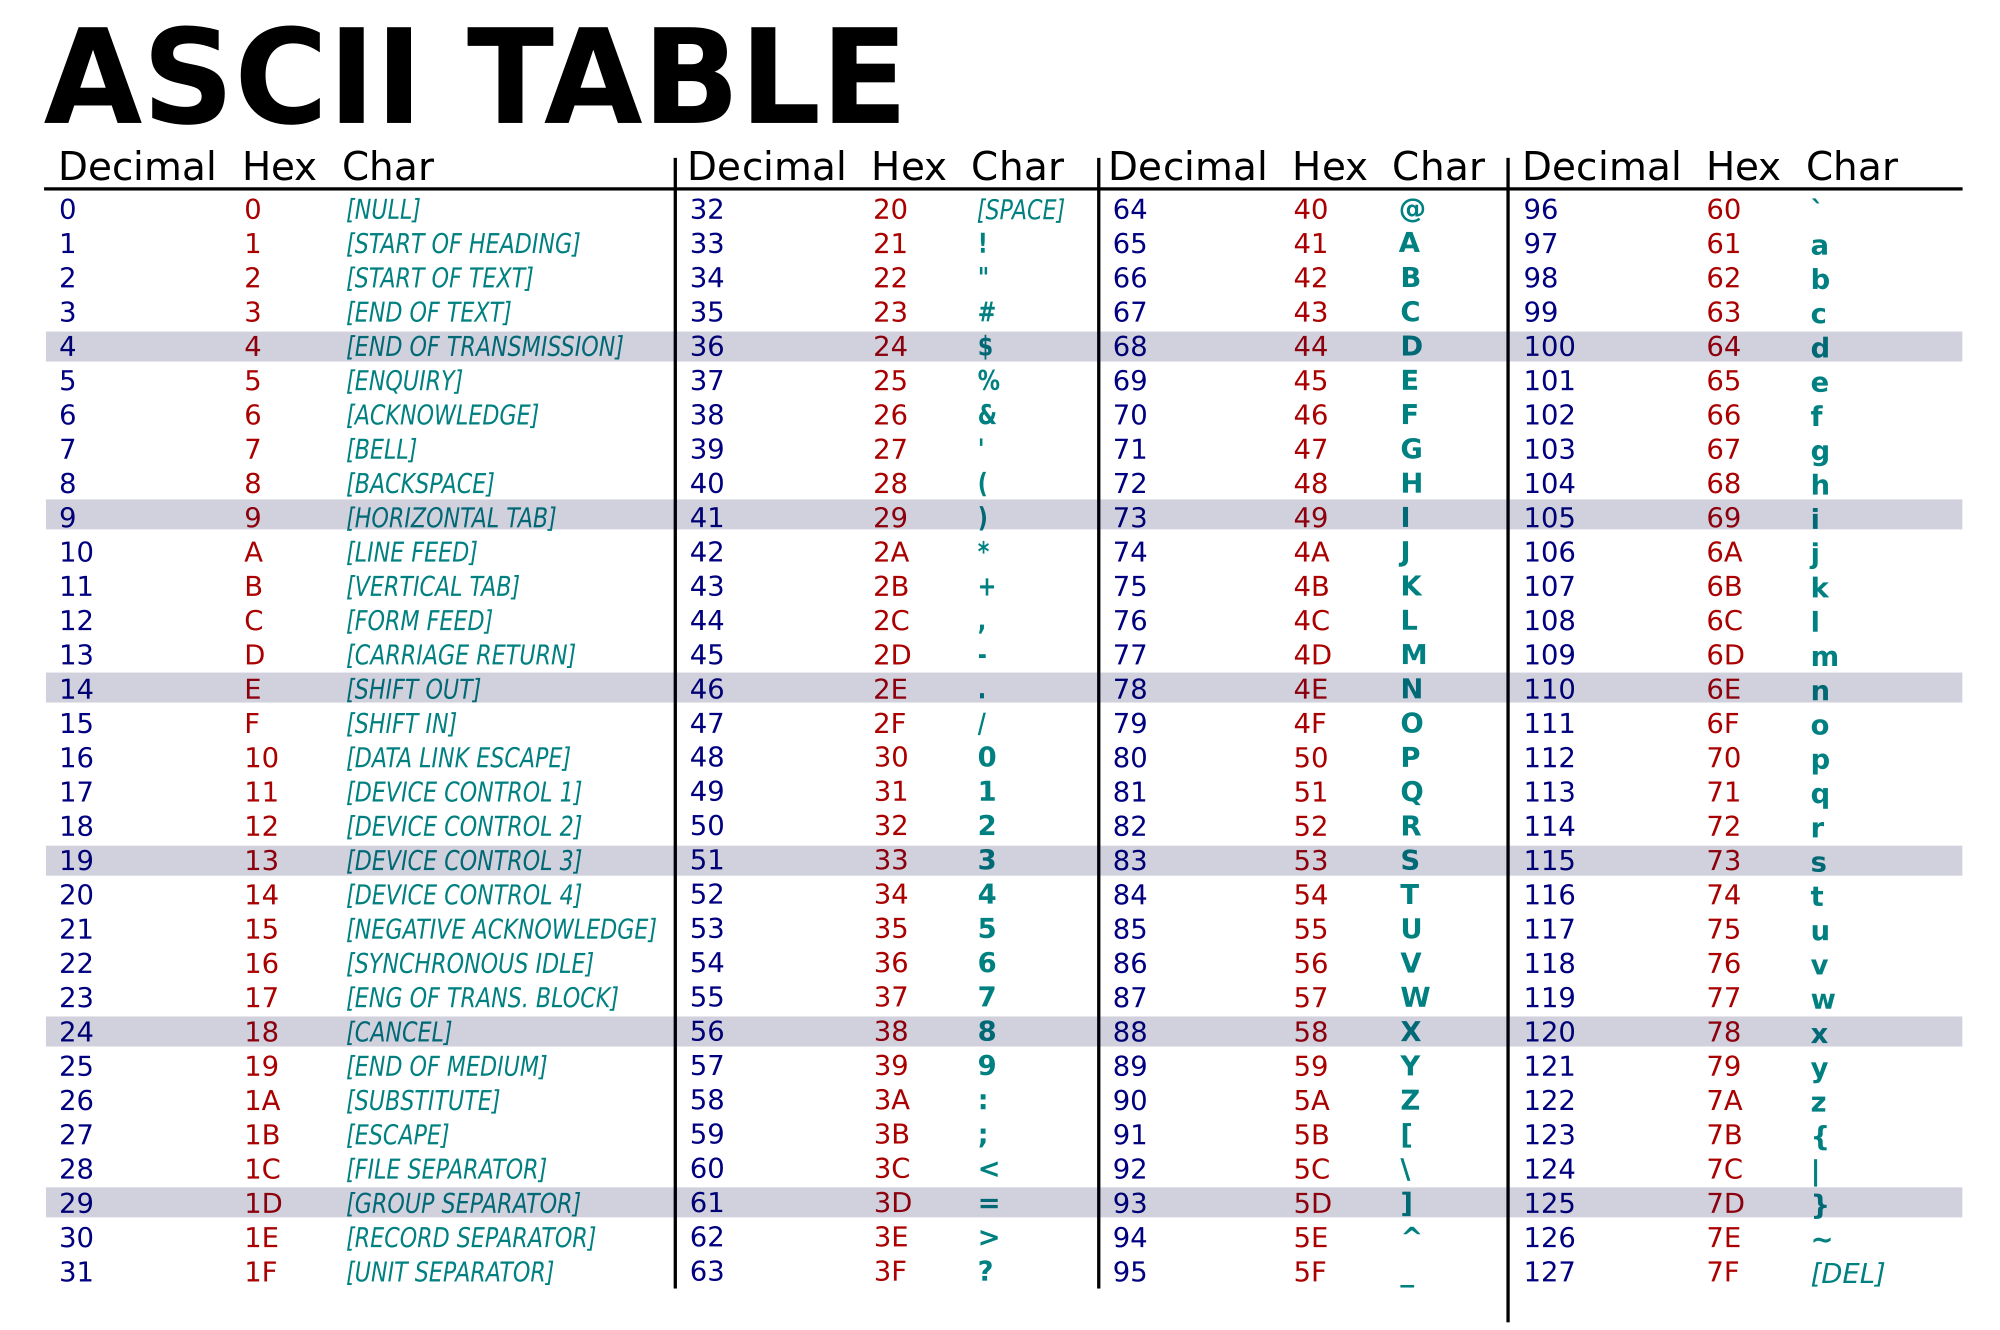
\includegraphics[width=130mm]{6_strings/ASCII.png}
\pagebreak

%%%%%%%%%%%%%%%%%%%%%%%%%%%%%%%%%%%%%%%%%%%%%%%%%%%%%%%%%%%%%%%%%%%%%%%%%%%%%%%%%%%%%%%%%
